\documentclass[a4paper, 14pt]{extreport}
\usepackage[T2A]{fontenc}
\usepackage[utf8]{inputenc}
\usepackage[english, russian]{babel}
\usepackage{indentfirst, setspace, titlesec, subcaption}
\usepackage{hyperref}
\usepackage{graphicx}
\usepackage{tocloft}
\usepackage[left=2.5cm, right=1.5cm, top=2.0cm, bottom=2.0cm]{geometry}

\graphicspath{{images/}}
\renewcommand{\rmdefault}{ftm}

\titleformat{\chapter}
    {\normalsize}
    {\thechapter}{1em}{}
\titleformat{\section}
    {\normalsize}
    {\thesection}{1em}{}
\titlespacing*{\chapter}{\parindent}{-30pt}{*2}
\titlespacing*{\paragraph}{\parindent}{-30pt}{*2}
\titlespacing*{\section}{\parindent}{*2}{*2}

\renewcommand{\cfttoctitlefont}{\normalfont\hspace{0.38\textwidth}}
\renewcommand{\cftchapleader}{\cftdotfill{\cftdotsep}}
\renewcommand{\cftbeforepartskip}{0em}
\renewcommand{\cftbeforechapskip}{0em}
\renewcommand{\cftchapfont}{\hspace{15pt}\normalsize}
\renewcommand{\cftsecfont}{\hspace{-6pt}}
\renewcommand{\cftsubsecfont}{\hspace{-38pt}}
\renewcommand{\cftchappagefont}{\normalfont}
\renewcommand{\cftbeforetoctitleskip}{-1em}
\renewcommand{\cftpartaftersnumb}{}
\renewcommand{\cftparskip}{-1mm}
\renewcommand{\cftdotsep}{2}

\begin{document}
    \begin{titlepage}
        \begin{center}
            Министерство образования и науки РФ \\
            Государственное образовательное учреждение\\
            Высшего профессионального образования\\
            <<Волгоградский государственный технический университет>>\\
            Кафедра <<САПР~и~ПК>>
        \end{center}
        \vspace{2.0cm}
        \begin{center}
            \large \textbf{ОТЧЁТ} \\
            по преддипломной практике \the\year г.
        \end{center}
        \begin{flushleft}
            Студента\\
            Фамилия \underline{Голубева\hspace{3.1cm}} 
            Имя \underline{Алексея\hspace{2.1cm}}\\
            Отчество \underline{Владимировича\hspace{1.6cm}}\\
            Факультет \underline{ФЭВТ\hspace{3.45cm}} курс \underline{2\hspace{1.5cm}} 
            группа \underline{САПР-2.1п\hspace{1.9cm}}\\
        \end{flushleft}
        \vspace{1.0cm}
        \noindentИндивидуальное задание: \underline{\hspace{22.3em}}\\
        \underline{\hspace{\textwidth}}
        \underline{\hspace{\textwidth}}
        \underline{\hspace{\textwidth}}
        \underline{\hspace{\textwidth}}
        \vspace{2.0cm}
        \begin{flushleft}
            РУКОВОДИТЕЛЬ\\
            Кафедра \underline{САПР~и~ПК\hspace{2.4cm}} Должность \underline{профессор\hspace{2.8cm}} \\
            Фамилия \underline{Кравец\hspace{3.3cm}} Имя \underline{Алла\hspace{5.5cm}}\\
            Отчество \underline{Григорьевна\hspace{2.2cm}}
        \end{flushleft}
        \vspace{1.5cm}
        \begin{flushright}
            <<\underline{\hspace{1.0cm}}>>\underline{\hspace{4.0cm}} \the\year г.
        \end{flushright}
        \vspace{\fill}
        \begin{center}
            Волгоград \the\year
        \end{center}
    \end{titlepage}
    \tableofcontents
    \onehalfspacing

    \chapter{Разработка методик тестирования системы построения маршрутов}
    \ldots

    \chapter{Произведение испытаний разработанной системы}
    \ldots

    \chapter{Результаты полученные в входе работы}
    % \vspace*{-2em}\begin{figure}[ht!]
    %     \center
    %     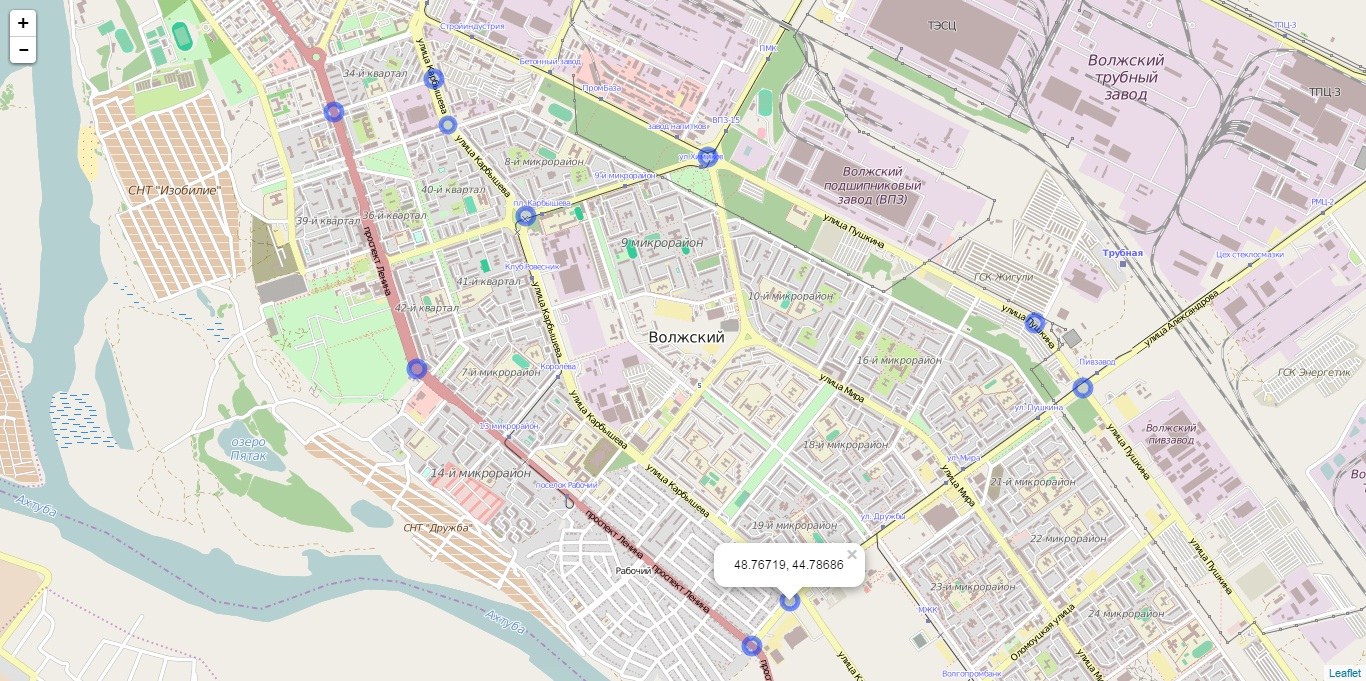
\includegraphics[width=0.55\textwidth]{e1}
    %     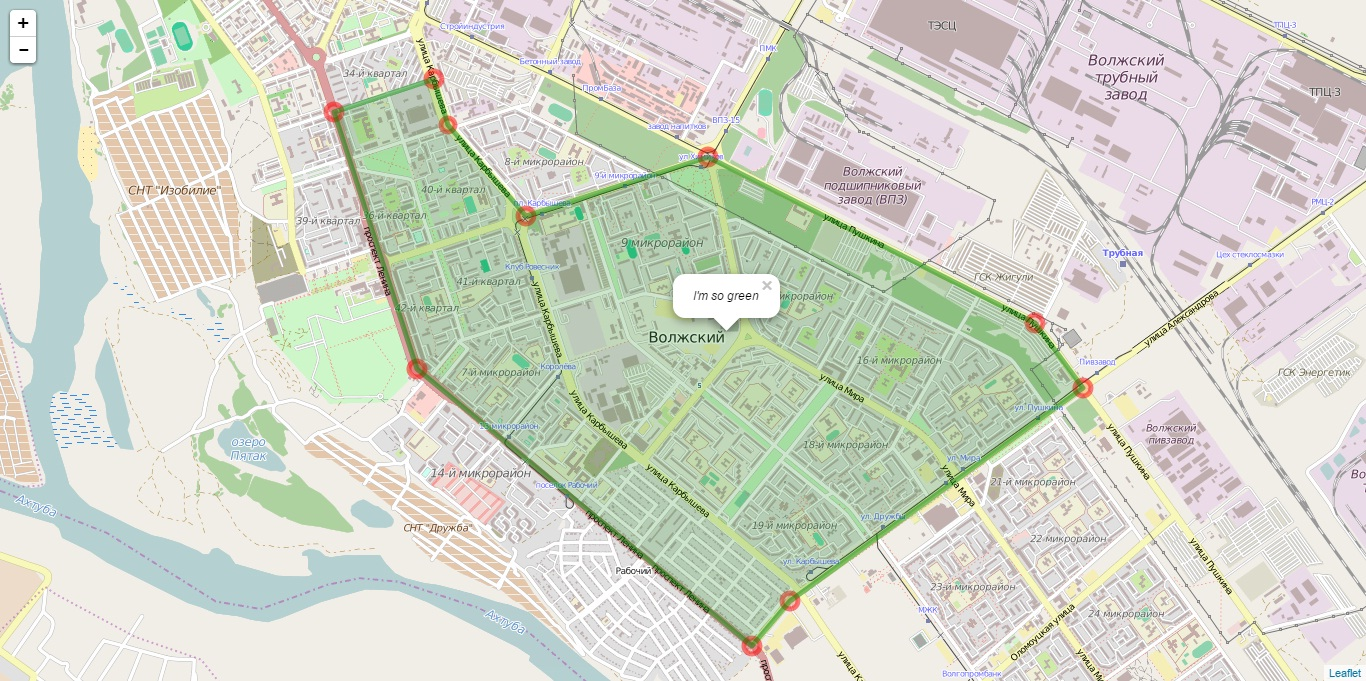
\includegraphics[width=0.55\textwidth]{e2}
    % \end{figure}

    \chapter{Структура четвёртой главы магистерской диссертации}
    В структуре четвёртой главый магистерской диссертации были выделены следующие пункты:
    % \begin{enumerate}
    %     \item Цель, задачи
    %     \item Теоретические положения
    %     \begin{enumerate}
    %         \item Технология OpenStreetMap
    %         \begin{enumerate}
    %             \item Введение
    %             \item Возможности
    %             \item Формат данных
    %         \end{enumerate}
    %         \item Библиотека Leaflet
    %         \begin{enumerate}
    %             \item Введение
    %             \item Возможности
    %         \end{enumerate}
    %     \end{enumerate}
    %     \item Пример выполнения лабораторной работы
    %     \begin{enumerate}
    %         \item Задача
    %         \item Подготовка HTML-страницы
    %         \item Создание карты
    %         \item Маркеры, круги и всплывающие сообщения
    %         \item Ломаная и область
    %     \end{enumerate}
    %     \item Задания на выполнение лабораторной работы
    %     \item Контрольные вопросы
    %     \item Литература
    % \end{enumerate}

    \newpage

    % В разделе <<Цель, задачи>> приводится цель лабораторной работы и общие
    % задачи, которые студент должен сделать во время ее выполнения.

    % В разделе <<Теоретические положения>> даётся общее описание технологии
    % OpenStreetMap, история возникновения и развития и используемый формат
    % данных. В этом же разделе даётся описание библиотеки Leaflet и ее
    % возможности.

    % В разделе <<Пример выполнения лабораторной работы>> студенту
    % предоставляются примеры выполнения простых заданий, снабженные подробным
    % описанием выполняемых действий: от подготовки HTML-страницы, до отображения
    % сложных структур данных. В нём подробно рассмотрено создание интерактивных
    % карт используя простой в реализации язык программирования Javascript.

    % В разделе <<Задания на выполнение лабораторной работы>> представлены
    % типовые задания для закрепления изученного материала лабораторной работы.

    % В разделе <<Контрольные вопросы>>~-- контрольные вопросы для проверки
    % теоретического минимума по данной теме.

    \chapter{Выводы по проделанной работе}
    В ходе преддипломной практики были выполнены следующие задачи:
    \begin{itemize}
        \item ...
    \end{itemize}

    \chapter{Используемые технологии в работе}
    Для проектирования и вёрстки были использованы следующие свободно распространяемые программные 
    продукты:
    \begin{itemize}
        \item Arch Linux -- это независимо разрабатываемый i686/x86-64 дистрибутив GNU/Linux общего 
            назначения \url{https://www.archlinux.org/}
        \item \TeX -- система компьютерной вёрстки, разработанная американским профессором информатики 
            Дональдом Кнутом в целях создания компьютерной типографии. \url{http://tug.org/}
        \item \LaTeX -- набор макрорасширений системы компьютерной вёрстки TeX.\\
            \url{http://www.latex-project.org/}
        \item Atom -- свободный открытый текстовой редактор исходных текстов программ.
            \url{https://atom.io/}
        \item Python -- высокоуровневый язык программирования общего назначения, ориентированный на повышение 
            производительности разработчика и читаемости кода. \url{https://www.python.org/}
        \item Matplotlib -- библиотека на языке программирования Python предназначенная для визуализации данных.
            \url{http://matplotlib.org/}
        \item Git -- распределённая система управления версиями файлов. Проект был создан Линусом 
            Торвальдсом для управления разработкой ядра Linux, первая версия выпущена 7 апреля 2005 года.\\
            \url{http://git-scm.com/}
        \item GitHub -- самый крупный веб-сервис для хостинга IT-проектов и их совместной разработки. 
            Основан на системе контроля версий Git и разработан на Ruby on Rails и Erlang компанией 
            GitHub, Inc.\\ \url{https://github.com/}
    \end{itemize}
\end{document}